% Source : http://forum.mathematex.net/latex-f6/barrer-un-paragraphe-t11503.html#p111622

\documentclass[10pt,a4paper]{article}
\usepackage[utf8x]{inputenc}
\usepackage{tikz}
\begin{document}
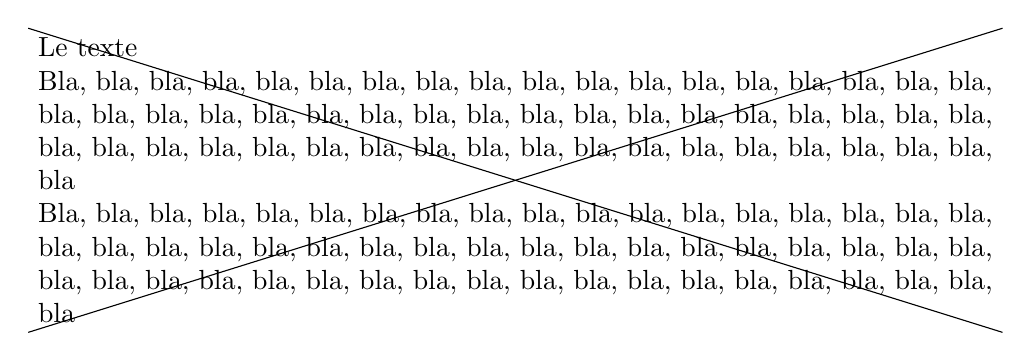
\begin{tikzpicture}
\node (box)
{
\begin{minipage}{\textwidth}
Le texte


Bla, bla, bla, bla, bla, bla, bla, bla, bla, bla, bla, bla, bla, bla, bla, bla, bla, bla, bla, bla, bla, bla, bla, bla, bla, bla, bla, bla, bla, bla, bla, bla, bla, bla, bla, bla, bla, bla, bla, bla, bla, bla, bla, bla, bla, bla, bla, bla, bla, bla, bla, bla, bla, bla, bla


Bla, bla, bla, bla, bla, bla, bla, bla, bla, bla, bla, bla, bla, bla, bla, bla, bla, bla, bla, bla, bla, bla, bla, bla, bla, bla, bla, bla, bla, bla, bla, bla, bla, bla, bla, bla, bla, bla, bla, bla, bla, bla, bla, bla, bla, bla, bla, bla, bla, bla, bla, bla, bla, bla, bla


\end{minipage}
};
\draw (box.north west) -- (box.south east); % pour un trait en diagonale principale
\draw (box.south west) -- (box.north east); % pour un autre trait en diagonale
\end{tikzpicture}
\end{document}